\section{Реализация}
В процессе работы над проектом было выделено две основных задачи: реализация
взаимодействия с пользователем и расширение функциональности для переформатирования программного текста с фильтрацией шаблонов.
%диаграмму что ли нарисавать?
Предполагаемый процесс взаимодействия с пользователем: пользователь выделяет
участок программного кода, в котором будут производиться изменение, и вызывает 
действие (Action), которое извлекает шаблон из выделенного участка
кода. Затем пользователь меняет форматирование этого же участка, выделяет его
снова и вызывает действие, которое извлекает новый шаблон форматирования и 
сохраняет его.

После этого происходит перепечатывание элементов (PsiElement), имеющих старое
форматирование, в файле, в котором пользователь менял программный текст.

\subsection{Переформатирование}
\subsubsection{Извлечение элемента для форматирования}
% тут будет диаграмма:
% 1) Получаем текст
% 2) Корректируем отступы + пример
% 3) Извлечение элемента (для того чтобы знать тип) -- вся рутина
% 4) Склеить текст и элемент
В первую очередь необходимо получить элемент, форматирование которого пользователь хочет изменить.
% Где-то надо ссылку на диаграмму, наверное, тут
Весь этот процесс изображен на рис.~\ref{fig:getElemDiag}.

\begin{figure}[h]
	\centering
	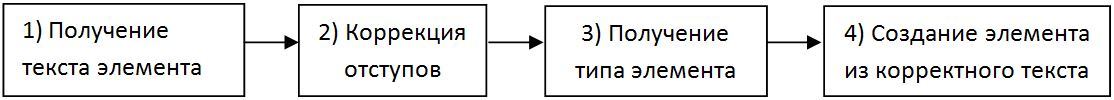
\includegraphics[width=\textwidth]{images/getElemDiag.jpg}
	\caption{Диаграмма этапов извлечения элемента из текста}
	\label{fig:getElemDiag}
\end{figure}

На первом этапе с помощью функций, предоставляемых IntelliJ IDEA API, можно получить текст элемента. 
Однако этот текст не всегда корректный, так как может содержать в себе лишние отступы.
Например, на рис. \ref{fig:offsetExample} изображены методы doSomething() и doAnotherThing(). 
Они имеют отступ относительно оператора ветвления, равный четырем пробелам.
Кроме того, они имеют отступ относительно метода foo(), равный восьми пробелам. 
Чтобы шаблон был корректным, на втором этапе убираются лишние пробелы (в данном случае четыре).
Далее получаем из текста сам элемент. 
Это необходимо, чтобы узнать его тип. %ссылку на дерево PsiElement'ов.
Затем (на четвертом этапе) из корректного текста и полученного элемента создается новый элемент того же типа, но с корректными отступами.

Все это необходимо проделать, так как IntelliJ IDEA API не предоставляет функционала по изменению текста элемента явным образом. 

\begin{figure}[h]
	\centering
	\lstinputlisting[language=C++]{codes/offsetExample.txt}
	\caption{Общий отступ элементов}
	\label{fig:offsetExample}
\end{figure}

Аналогичные действия необходимо повторить для получения элемента из измененного
пользователем текста. 
Из этого элемента извлекается шаблон и сохраняется принтером для дальнейшего использования.

%\subsubsection{Извлечение шаблона}
%Шаблон, как и прежде, извлекается методами класса \lstinline[language=C++]{PsiElementComponent}.

%\subsubsection{Добавление шаблона}
%В связи с тем, что возникла необходимость добавления одного шаблона, класс %Printer обзавелся публичным методом, реализующим этот процесс. Остальные
%действия аналогичны тем при заполнении списка шаблонов из файла.

\subsubsection{Сравнение с шаблоном}
Как уже было отмечено в обзоре, при перепечатывании принтер обходит все элементы (PsiElement) дерева разбора и применяет к ним новые шаблоны. 
В рамках реализуемого подхода происходит перепечатывание лишь тех элементов, которые имели старое форматирование.
Это необходимо, если хочется поддерживать два и более различных варианта форматирования элементов некоторого типа. 
На рис. \ref{templates} изображены три блока оператора ветвления. 
Без фильтрации шаблонов все три блока будут изменены и получат одинаковое форматирование. %рис. сделать 
Однако первые два блока и так легко читаемы и понятны. 
Третий блок, будучи однострочным, уже не будет восприниматься так же хорошо.
Кроме того, существуют ограничения на ширину вывода, то есть в одной строке не можеть быть символов больше некоторой наперед заданной величины.

%\begin{figure}[t]
%    \centering
%    \lstinputlisting[language=C++]{codes/sameTmpltElems.txt}
%    \caption{Шаблоны}
%    \label{fig:sameTmpltElems}
%\end{figure}
%добавить вторую картинку как стало бы
\fvset{frame=lines,framesep=7pt}
\begin{figure}[ht]
\noindent\begin{minipage}{.5\textwidth}
    \lstinputlisting[language=C++]{codes/sameTmpltElems.txt}
\caption*{а) До переформатирования}    
\end{minipage}\hfill
\begin{minipage}{.5\textwidth}
    \lstinputlisting[language=C++]{codes/sameTmpltElems2.txt}
\caption*{б) После переформатирования}    
\end{minipage}
\caption{Переформатирование элементов одного типа без фильтрации шаблонов} 
\label{templates}
\end{figure}


Чтобы сделать настройку форматирования более гибкой и избавиться от подобного рода проблем, необходимо производить сравнение шаблонов текущего элемента дерева разбора и элемента со старым форматированием. 
Переформатировать элемент -- только в случае совпадения шаблонов.
Шаблоны совпадают, если совпадет их текстовое представление: шаблон записывается в виде строки, которая содержит необходимые элементы: ключевые слова, пробелы, переносы строк, скобки, а так же метки для поддеревьев, в которых указывается дополнительная информация, например, количество выражений в поддереве (одно или несколько).
В случае оператора ветвления (рис.~\ref{iftmpltcode}а) его поддеревьями являются: условие (condition), ветка, соответствующая выполнению условия (then block) и содержащая несколько подвыражений, ветка, соответствующая невыполнению условия (else block) и содержащая одно подвыражение. %ifTmplt ifTmpltCode
Соответствующий ему шаблон изображен на рисунке~\ref{iftmpltcode}б.
\fvset{frame=lines,framesep=7pt}
\begin{figure}[ht]
\noindent\begin{minipage}{.5\textwidth}
    \lstinputlisting[language=C++]{codes/ifTmpltCode.txt}
\caption*{а) Оператор ветвления}    
\end{minipage}\hfill
\begin{minipage}{.5\textwidth}
    \lstinputlisting[language=C++]{codes/ifTmplt.txt}
\caption*{б) Шаблон для оператора ветвления}    
\end{minipage}
\caption{Оператор ветвления и соответствующий ему шаблон}    
\label{iftmpltcode}
\end{figure}

%\begin{figure}[t]
%    \centering
%    \lstinputlisting[language=C++]{codes/sameTmpltElems.txt}
%    \caption{Шаблоны}
%    \label{fig:sameTmpltElems}
%\end{figure}
%добавить вторую картинку как стало бы

\subsection{Оценка производительности}
Описанный выше способ  давал очень низкую производительность. 
В таблице~\ref{table:slow} приведено время, затрачиваемое принтером на переформатирование файлов различной длины. 
Измерения производились на примере двух блоков: оператора ветвления и метода.

\begin{table}[h]
\begin{tabular}{cc|c|c|c|c|}
\cline{2-5}
\multicolumn{1}{ c| }{ } & \multicolumn{2}{p{6cm} |}{Формат. операторов ветвления} & \multicolumn{2}{p{5cm} |}{Форматирование методов} \\
\hline
\multicolumn{1}{ |c| }{Размер файла (строк)} & Кол-во & Время (сек.) & Кол-во & Время (сек.) \\ 
\hline
\multicolumn{1}{ |c| }{>7000}           & 520   & 35    & 660  & 58 \\
\multicolumn{1}{ |c| }{1000..2000}       & 145   & 2.7   & 90   & 4.4 \\
\multicolumn{1}{ |c| }{500..1000}       & 54    & 0.73  & 72   & 1.34 \\
\multicolumn{1}{ |c| }{0..500}          & 35    & 0.2   & 36   & 0.67 \\
\hline
\end{tabular}
\caption{Время переформатирования файлов I}
\label{table:slow}
\end{table}


Причина столь низкой производительности кроется в том, что для переформатирования элементов используется тот же способ, что и при форматировании по образцу:
принтер обходит все дерево разбора и сравнивает шаблоны.
%Однако нет необходимости проверять на совпадение шаблоны, полученные из каждого элемента дерева разбора, и шаблон, полученного из элемента со старым форматированием.
Однако нет необходимости сравнивать шаблон, полученный из элемента со старым форматированием, с шаблоном, полученным из каждого элемента дерева разбора.
Количество вариантов для переформатирования можно сузить лишь для элементов того же типа.

Для уменьшения затрат времени при обходе дерева элементов создается список кандидатов на форматирование (элементы того же типа, что и элемент со старым форматированием). 
После этого из элементов созданного списка извлекаются шаблоны.
Если полученный шаблон совпадает с шаблоном элемента со старым форматированием, то происходит перепечатывание элемента и замена его в дереве разбора.
Время, затрачиваемое в этом случае на переформатирование, приведено в таблице~\ref{table:fast}.

%\begin{table}[h]
%\begin{tabular}{ l | p{4cm} | p{4cm} }
%  Размер файла (строк) & Формат. операторов ветвления (сек.) & Формат. методов %(сек.) \\ 
%  \hline
%  >7000         & 6.6   & 5.8 \\
%  1000..2000    & 0.72  & 1   \\
%  500..1000     & 0.125 & 0.67 \\
%  0..500        & 0.145 & 0.325 \\
%\end{tabular}
%\caption{Время переформатирования файлов II}
%\label{table:fast}
%\end{table}


\begin{table}[h]
\begin{tabular}{cc|c|c|c|c|}
\cline{2-5}
\multicolumn{1}{ c| }{ } & \multicolumn{2}{p{6cm} |}{Формат. операторов ветвления} & \multicolumn{2}{p{5cm} |}{Форматирование  методов} \\
\hline
\multicolumn{1}{ |c| }{Размер файла (строк)} & Кол-во & Время (сек.) & Кол-во & Время (сек.) \\ 
\hline
\multicolumn{1}{ |c| }{>7000}           & 520   & 6.6   & 660  & 5.8 \\
\multicolumn{1}{ |c| }{1000..2000}      & 145   & 0.72  & 90   & 1 \\
\multicolumn{1}{ |c| }{500..1000}       & 54    & 0.225 & 72   & 0.67 \\
\multicolumn{1}{ |c| }{0..500}          & 35    & 0.145 & 36   & 0.325 \\
\hline
\end{tabular}
\caption{Время переформатирования файлов II}
\label{table:fast}
\end{table}